% !TeX root = ../wireless_networks.tex

\chapter{Wireless Networks}

\section{Wireless Network}
Wireless is a term used to describe telecommunications in which electromagnetic waves carry the signal. A wireless network is defined as technology that allows two or more computers to communicate, using standard protocol but without the use of network cabling. A wireless LAN (or WLAN) is one in which a mobile user can connect to a local area network through a wireless (radio) connection. The IEEE 802.11 group of standards specifies the technologies for wireless LANs.

\section{Wireless Network Architecture}
WLAN consist of two main components: 
\begin{itemize}
	\item An Access Point (AP) and wireless adapters.
	\item An access point looks like an	external modem with two small antennae.
	\item Radio cards are also called WLAN cards. 
	\item The range of an 802.11b WLAN is typically 100 feet and can be extended
	to several hundred feet by using an antenna. 
	\item Wireless bridges are similar to the wired bridges and are used to connect two WLANs.
\end{itemize}

See Section \ref{sec:wireless-network-architecture} for explanation.
 
\section{Wireless Switching Technology}
Switching is process to forward packets coming in from one port to a port leading towards the
destination. When data comes on a port it is called ingress, and when data leaves a port or goes out it
is called egress. A communication system may include number of switches and nodes.

\subsection{Circuit Switching}
\begin{multicols}{2}
	\begin{itemize}
		\item When two nodes communicate with each other over a dedicated communication path, it is called
		circuit switching.
		\item There is a need of pre-specified route from which data travels and no other data is permitted.
		\item In circuit switching, to transfer the data, circuit must be established so that the data transfer can take place.
		\item Circuit switching was designed for voice applications.
		
		\item Telephone is the best suitable example of circuit switching. Before a user can make a call, a virtual path between caller and call receiver person is established over the network.
	\end{itemize}
\end{multicols}


\begin{figure}[hpt]
	\begin{center}
		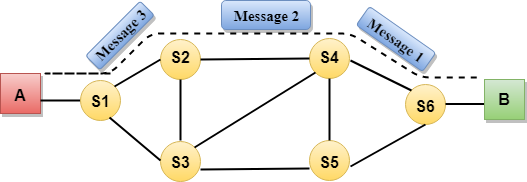
\includegraphics[width=0.8\textwidth]{circuit-switching}
		\caption{Circuit switching}
		\label{fig:circuit-switching}
	\end{center}
\end{figure}
%-------------------FIGURE END----------------------

\textit{Circuits can be permanent or temporary. Applications which use circuit switching may have to go through three phases:}

\begin{multicols}{3}
	\begin{enumerate}[label=\alph*.]
		\item Establish a circuit
		\item Transfer the data
		\item Disconnect the circuit
	\end{enumerate}
\end{multicols}



\begin{multicols}{2}
	\subsubsection*{Advantages}
	\begin{itemize}
		\item In the case of Circuit Switching technique, the communication channel is dedicated.
		\item It has fixed bandwidth.
	\end{itemize}
\end{multicols}



\begin{multicols}{2}
\subsubsection*{Disadvantages}
	\begin{itemize}
		\item Once the dedicated path is established, the only delay occurs in the speed of data transmission.
		\item It takes a long time to establish a connection approx 10 seconds during which no data can be transmitted.
		\item It is more expensive than other switching techniques as a dedicated path is required for each connection.
		\item It is inefficient to use because once the path is established and no data is transferred, then the capacity of the path is wasted.
		\item In this case, the connection is dedicated therefore no other data can be transferred even if the channel is free.
	\end{itemize}
\end{multicols}


\subsection{Message Switching}
\begin{multicols}{2}
	\begin{itemize}
		\item This technique was somewhere in the middle of circuit switching and packet switching.
		\item In message switching, the whole message is treated as a data unit and is switching / transferred in its entirety.
		
		\item A switch working on message switching, first receives the whole message and buffers it until there are resources available to transfer it to the next hop.
		\item If the next hop is not having enough resource to accommodate large size message, the message is stored and switch waits.
		\item This technique was considered substitute to circuit switching.
		\item As in circuit switching, the whole path is blocked for two entities only.
		\item Message switching is replaced by packet switching.
	\end{itemize}
\end{multicols}


%---------------------------------------------------
%
%				FIGURE
%
%---------------------------------------------------
\begin{figure}[pht]
	\begin{center}
		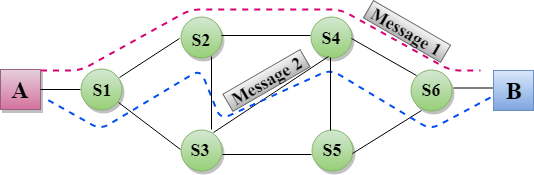
\includegraphics[width=0.8\textwidth]{message-switching}
		\caption{Message switching}
		\label{fig:message-switching}
	\end{center}
\end{figure}
%-------------------FIGURE END----------------------

%Message switching has the following drawbacks:
%\begin{itemize}
%	\item Every switch in transit path needs enough storage to accommodate entire message.
%	\item Because of store-and-forward technique and waits included until resources are available,
%	message switching is very slow.
%	\item Message switching was not a solution for streaming media and real-time applications.
%\end{itemize}


\begin{multicols}{2}
	\subsubsection*{Advantages}
	\begin{itemize}
		\item Data channels are shared among the communicating devices that improve the efficiency of using available bandwidth.
		\item Traffic congestion can be reduced because the message is temporarily stored in the nodes.
		\item Message priority can be used to manage the network.
		\item The size of the message which is sent over the network can be varied. Therefore, it supports the data of unlimited size.
	\end{itemize}
\end{multicols}


\subsubsection*{Disadvantages}
\begin{multicols}{2}
	\begin{itemize}
		\item The message switches must be equipped with sufficient storage to enable them to store the messages until the message is forwarded.
		\item The Long delay can occur due to the storing and forwarding facility provided by the message switching technique.
	\end{itemize}
\end{multicols}



\begin{multicols}{2}
	\subsection{Packet Switching}
	\begin{itemize}
		\item Shortcomings of message switching gave birth to an idea of packet switching.
		\item The entire message is broken down into smaller chunks called packets.
		\item The switching information is added in the header of each packet and transmitted independently.
		\item It is easier for intermediate networking devices to store small size packets, and they do not take much resources either on carrier path or in the internal memory of switches.
		Packet switching enhances line efficiency
		as packets from multiple applications can
		be multiplexed over the carrier.
		\item The Internet uses packet switching technique. Packet switching enables the user to differentiate data streams based on priorities.
		\item Packets are stored and forwarded according to their priority to provide quality of service.
	\end{itemize}
\end{multicols}


%---------------------------------------------------
%				FIGURE
%---------------------------------------------------

\begin{figure}[hpb!]
	\begin{center}
		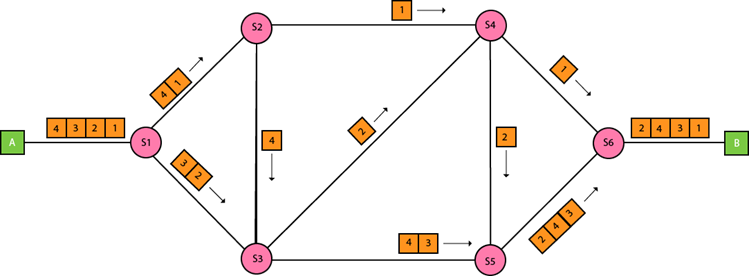
\includegraphics[width=0.8\textwidth]{packet-switching}
		\caption{Packet switching}
		\label{fig:packet-switching}
	\end{center}
\end{figure}
%-------------------FIGURE END----------------------
\raggedbottom

\begin{multicols}{2}
	\subsubsection*{Advantages}
	\begin{itemize}
		\item \textit{Cost-effective}: In packet switching technique, switching devices do not require massive secondary storage to store the packets, so cost is minimized to some extent. Therefore, we can say that the packet switching technique is a cost-effective technique.
		\item \textit{Reliable}: If any node is busy, then the packets can be rerouted. This ensures that the Packet Switching technique provides reliable communication.
		\item \textit{Efficient}: Packet Switching is an efficient technique. It does not require any established path prior to the transmission, and many users can use the same communication channel simultaneously, hence makes use of available bandwidth very efficiently.
	\end{itemize}
\end{multicols}


\begin{multicols}{2}
	\subsubsection*{Disadvantages}
	\begin{itemize}
		\item Packet Switching technique cannot be implemented in those applications that require low delay and high-quality services.
		\item The protocols used in a packet switching technique are very complex and requires high implementation cost.
		\item If the network is overloaded or corrupted, then it requires re-transmission of lost packets. It can also lead to the loss of critical information if errors are not recovered.
	\end{itemize}
\end{multicols}


\begin{table}[hpt!]
	\centering
	\caption{Differences between circuit switching and packet switching}
	\label{tab:circut-vs-packet}
	\begin{center}
		\begin{tabular}{p{5cm}p{5cm}}
		\toprule	
		\textbf{Circuit Switching}	& \textbf{ Packet Switching} \\
		
		\midrule
		Physical path between source and destination	& No physical path\\
		All packets use same path & Packets travels independently \\
		Bandwidth wastage & No bandwidth wastage	\\
		More reliable & Less reliable\\
		No store and forward transmission	& Supports store and forward transmission\\
		\bottomrule
	\end{tabular}
	\end{center}
\end{table}

\section{Wireless Communication Problem}

\subsection{Interference}
\begin{itemize}
	\item Radio transmission cannot be protected against interference using shielding as this is done in coaxial cable or shielded twisted pair. 
	\item For example, electrical engines and lightning cause severe interference and result in higher loss rates for transmitted data or higher bit error rates respectively.
\end{itemize}

\subsection{Regulations and Spectrum}
Frequencies have to be coordinated, and unfortunately, only a very limited amount of frequencies are available  

\subsection{Low Bandwidth}
Transmission rates are very low for wireless devices compared to desktop systems.

\subsection{High Delays}
A serious problem for communication protocols used in today’s Internet (TCP/IP) is the big variation in link characteristics. 

\subsection{Lower Security}
Not only can portable devices be stolen more easily, but the radio interface is also prone to the dangers of eavesdropping.

\subsection{Shared Medium}
Radio access is always realized via a shared medium. As it is impossible to have a separate wire between a sender and each receiver, different competitors have to ‘fight’ for the medium. 

\section{Wireless Network Reference Model}
The architecture of a network defines the protocols and components necessary to satisfy application requirements. One popular standard for illustrating the architecture is the
seven-layer Open System Interconnect (OSI) Reference Model, developed by the International Standards Organization (ISO). OSI specifies a complete set of network functions, grouped into layers, which reside within each network component. The OSI Reference Model is also a handy model for representing the various standards and interoperability of a wireless network.


\begin{figure}[tph]
	\centering
	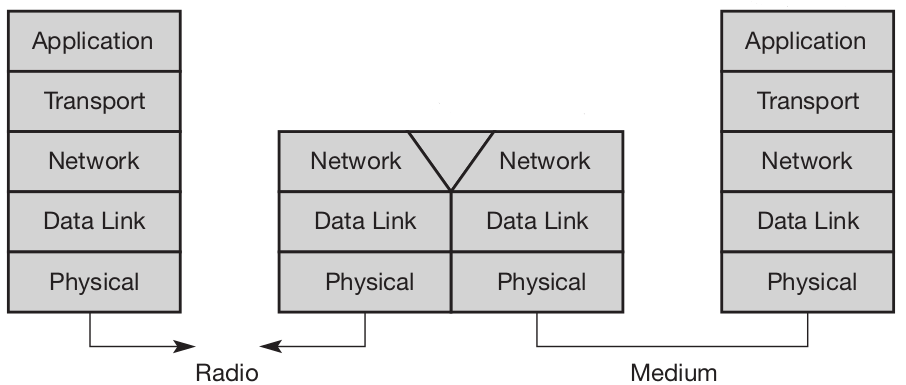
\includegraphics[width=0.8\textwidth]{graphics/wireless-ref-model}
	\caption{Wireless Network Reference Model}
	\label{fig:wireless-ref-model}
\end{figure}



The OSI layers provide the following network functionality:

\subsection*{Layer 7 - Application Layer}
\begin{itemize}
	\item Establishes communications among users and provides basic communications services such as file transfer and e-mail. 
	\item Examples of software that runs at this layer include Simple Mail Transfer Protocol (SMTP), HyperText Transfer Protocol (HTTP) and File Transfer Protocol (FTP).
\end{itemize}


\subsection*{Layer 6 - Presentation Layer} 
\begin{itemize}
	\item Negotiates data transfer syntax for the application layer and performs translations between different data formats, if necessary. 
	\item For example, this layer can translate the coding that represents the data when communicating with a remote system made by a different vendor. 
\end{itemize}


\subsection*{Layer 5 - Session layer}
\begin{itemize}
	\item Establishes, manages, and terminates sessions between applications. Wireless middleware and access controllers provide this form of connectivity over wireless networks. 
	\item If the wireless network encounters interference, the session layer functions will suspend communications until the interference goes away.
\end{itemize}


\subsection*{Layer 4 - Transport Layer}
\begin{itemize}
	\item Provides mechanisms for the establishment, maintenance, and orderly termination of virtual circuits, while shielding the higher layers from the network implementation details. 
	\item In general, these circuits are connections made between network applications from one end of the communications circuit to another (such as between the web browser on a laptop to a web page on a server). 
	\item Protocols such as Transmission Control Protocol (TCP) operate at this layer. 
\end{itemize}


\subsection*{Layer 3 - Network Layer}
\begin{itemize}
	\item Provides the routing of packets though a network from source to destination. 
	\item This routing ensures that data packets are sent in a direction that leads to a particular destination. 
	\item Protocols such as Internet Protocol (IP) operate at this layer.
\end{itemize}


\subsection*{Layer 2 - Data link Layer}
\begin{itemize}
	\item Ensures medium access, as well as synchronization and error control between two entities. 
	\item With wireless networks, this often involves coordination of access to the common air medium and recovery from errors that might occur in the data as it propagates from source to destination. 
	\item Most wireless network types have a common method of performing data link layer functions independent of the actual means of transmission.
\end{itemize}


\subsection*{Layer 1 - Physical Layer}
\begin{itemize}
	\item Provides the actual transmission of information through the medium. 
	\item Physical layers include radio waves and infrared light. 
\end{itemize}

\noindent The combined layers of a network architecture define the functionality of a wireless network, but wireless networks directly implement only the lower layers of the model. A wireless NIC, for example, implements the data link layer and physical layer functions. Other elements of the network (such as wireless middleware), however, offer functions that the session layer implements. In some cases, the addition of a wireless network might impact only the lower layers, but attention to higher layers is necessary to ensure that applications operate effectively in the presence of wireless network impairments. 

Each layer of the OSI model supports the layers above it. In fact, the lower layers often appear transparent to the layers above. For example, TCP operating at the transport layer establishes connections with applications at a distant host computer, without awareness
that lower layers are taking care of synchronization and signaling. 

\section{Wireless Networking Issues \& Standards}

\subsection{Wireless Networking Issues}
\begin{multicols}{2}
%	\begin{itemize}
%		\item Higher loss-rates due to interference (emissions of, e.g., engines, lightning)
%		
%		\item Restrictive regulations of frequencies: frequencies have to be coordinated, useful frequencies are almost all occupied
%		
%		\item Low data transmission rates: local some Mbit/s, regional currently, e.g., 53kbit/s with GSM/ GPRS
%		
%		\item Higher delays, higher jitter: connection setup time with GSM in the second range, several hundred
%		milliseconds for other wireless systems
%		
%		\item Lower security, simpler active attacking: radio interface accessible for everyone, base station can be simulated,
%		thus attracting calls from mobile phones
%		
%		\item Quality of Service (QoS): One of the primary concerns about wireless
%		data delivery is that, unlike the Internet through wired services, QoS is
%		inadequate. Lost packets and atmospheric interference are recurring
%		problems of the wireless protocols.
%		
%		\item Security risk: This is another major issue with a data transfer over a
%		wireless network. Basic network security mechanisms like the service set
%		identifier (SSID) and Wireless Equivalency Privacy (WEP);these measures
%		may be adequate for residences and small businesses, but they are
%		inadequate for the entities that require stronger security.
%	\end{itemize}
\begin{itemize}
	
	\item \textbf{Quality of service}: WLANs typically offer lower quality than their wired counterparts. The main reasons for this are the lower bandwidth due to limitations in radio transmission, and higher delay variation due to extensive error correction and detection mechanisms.
	
	
	
	\item \textbf{Proprietary solutions}: Due to slow standardization procedures, many companies have come up with proprietary solutions offering standardized functionality plus many enhanced features. However, these additional features only work in a homogeneous environment, i.\ e.\ , when adapters from the same vendors are used for all wireless nodes.
	
	
	\item \textbf{Restrictions}: All wireless products have to comply with national regulations. Several government and non-government institutions worldwide regulate the operation and restrict frequencies to minimize interference. WLANs are limited to low-power senders and certain license-free frequency bands, which are not the same worldwide.
	
	\item \textbf{Safety and security}: Using radio waves for data transmission might interfere with other high-tech equipment in, e.\ g.\ , hospitals. Senders and
	receivers are operated by laymen and, radiation has to be low. Special precautions have to be taken to prevent safety hazards. The open radio interface makes eavesdropping much easier in WLANs than, e.\ g.\ , in the case of fiber optics.
	
\end{itemize}
\end{multicols}



\subsection{Wireless Networking Standards}

802.11 represents the IEEE designation for wireless networking. Several wireless networking specifications exist under the 802.11 banner. The 802.11 wireless standards can differ in terms of speed, transmission ranges, and frequency used, but
in terms of actual implementation they are similar. All standards can use either an
infrastructure or ad hoc network design, and each can use the same security
protocols.

\subsubsection*{IEEE 802.11}
\begin{itemize}
	\item There were actually two variations on the initial 802.11 wireless standard.
	\item Both offered $ 1 $ or $ 2Mbps $ transmission speeds and the same RF of $ 2.4GHz $.
	\item The difference between the two was in how data traveled through the RF media. 
	\begin{itemize}
		\item one used FHSS (Frequency Hopping Spread Spectrum), and the 
		\item other used DSSS (Direct Sequence Spread Spectrum). 
	\end{itemize}
	\item The original 802.11 standards are far too slow for modern networking needs and are now no longer deployed.
\end{itemize}

\paragraph*{IEEE 802.11a}
\begin{itemize}
	\item In terms of speed, the 802.11a standard was far ahead of the original 802.11 standards. 
	\item 802.11a specified speeds of up to $ 54Mbps $ in the $ 5GHz $ band.
	\item 802.11a is incompatible with the 802.11b and 802.11g wireless standards.
\end{itemize}

\paragraph*{IEEE 802.11b}
\begin{itemize}
	\item The 802.11b standard provides for a maximum transmission speed of $ 11Mbps $. 
	\item Devices are designed to be backward-compatible with previous 802.11 standards
	\item 802.11b uses a $ 2.4GHz $ RF range and is compatible with 802.11g.
\end{itemize}


\paragraph*{IEEE 802.11g}
\begin{itemize}
	\item 802.11g is a popular wireless standard today. 
	\item 802.11g offers wireless transmission over distances of $ 150 feet $ and speeds up to $  54Mbps $
	\item 802.11g operates in the $ 2.4GHz $ range and therefore is compatible with it.
\end{itemize}


\paragraph*{IEEE 802.11n}
\begin{itemize}
	\item The newest of the wireless standards listed is 802.11n. 
	\item The goal of the 802.11n standard is to significantly increase throughput in both the $ 2.4GHz $ and the $ 5GHz $ frequency range. 
	\item The baseline goal of the standard was to reach speeds of $ 100Mbps $.
	\item Given the right conditions, speeds might reach a $ 600Mbps $. 
	\item In practical operation, 802.11n speeds is much slower.
\end{itemize}



\section{Mobile Computing}
Mobile Computing is a technology that allows transmission of data, voice and video via a computer or any other wireless enabled device without having to be connected to a fixed physical link. 

\subsection{Mobile Communication}
Mobile Communication is a wireless form of communication in which
voice and data information is emitted, transmitted and received via
microwaves. This type of communication allows individuals to
converse with one another and/or transmit and receive data while
moving from place to place. Some examples include: cellular and
digital cordless telephones, pagers, telephone answering devices,
air-to-ground telecommunications and satellite-based
communications.


\subsection{Principles of Mobile Computing}
\begin{itemize}
\item \textbf{Portability}: Devices/nodes connected within the mobile computing
system should facilitate mobility. These devices may have limited
device capabilities and limited power supply, but should have a
sufficient processing capability and physical portability to operate in a
movable environment.

\item \textbf{Connectivity}: This defines the quality of service (QoS) of the network
connectivity. In a mobile computing system, the network availability is
expected to be maintained at a high level with the minimal amount of
lag/downtime without being affected by the mobility of the connected
nodes.

\item \textbf{Interactivity}: The nodes belonging to a mobile computing system are
connected with one another to communicate and collaborate through
active transactions of data.

\item \textbf{Individuality}: A portable device or a mobile node connected to a mobile
network often denote an individual; a mobile computing system should
be able to adopt the technology to cater the individual needs and also
to obtain contextual information of each node.
\end{itemize}



\subsection{Mobile Computing Architecture}
%\begin{figure}[pht]
%	\centering
%	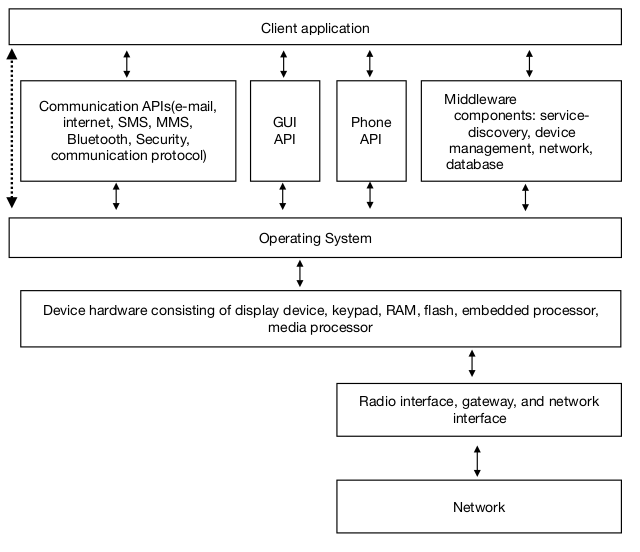
\includegraphics[width=0.8\textwidth]{mobile-computing-architecture}
%	\caption{Mobile Computing Architecture.}
%\end{figure}
The network-centric mobile computing architecture uses three-tier architecture as shown in Figure \ref{fig:3-tier-mobile-computing-architecture}.
\begin{enumerate}
	\item \textit{Tier-1} : Presentation Tier / User interface 
	\item \textit{Tier-2} : Application Tier / Process Management Tier
	\item \textit{Tier-2} : Data Tier / Database Management Tier
\end{enumerate}

%---------------------------------------------------
%				FIGURE
%---------------------------------------------------
\begin{figure}[hpt]
	\begin{center}
		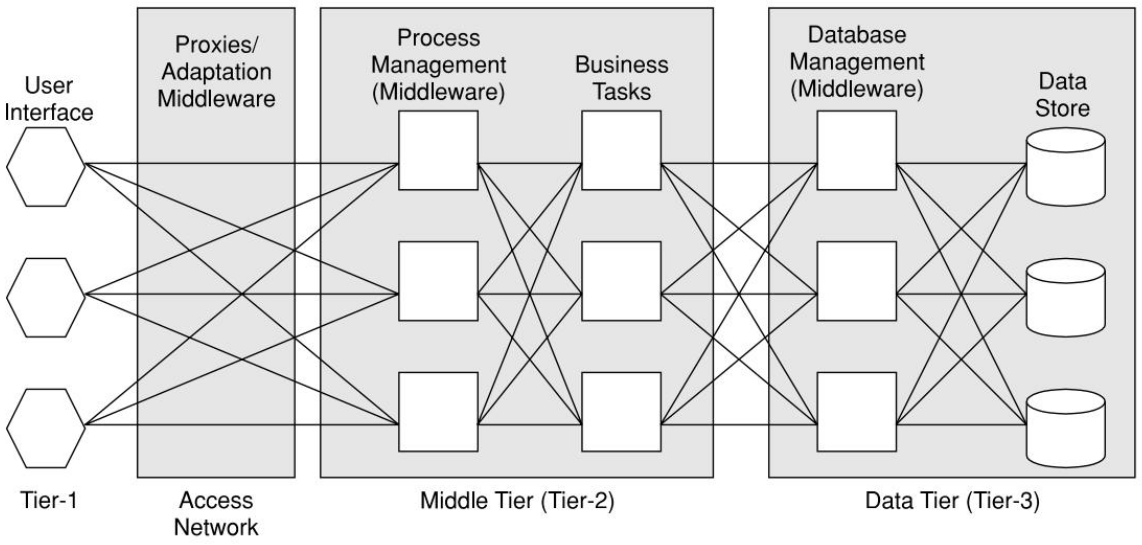
\includegraphics[width=0.9\textwidth]{3-tier-mobile-computing-architecture}
		\caption{Three-tier architecture for mobile computing}
		\label{fig:3-tier-mobile-computing-architecture}
	\end{center}
\end{figure}


\begin{multicols}{2}
	\subsubsection{Presentation Tier}
	\begin{itemize}
		\item This is the user facing system in the first tier. 
		\item This is the layer of agent applications and systems which run on the client device and offer all the user interfaces.
		\item These applications run on the client device and offer all the user interfaces. 
		\item This tier is responsible for presenting the information to the end user.
		\item This tier includes web browsers and customized client programs. 
	\end{itemize}
\end{multicols}


\begin{multicols}{2}
	\subsubsection{Application Tier}
	\begin{itemize}
		\item The application tier or middle tier is the ``engine'' of a ubiquitous application. 
		\item It performs the business logic of processing user input, obtaining data, and making decisions. 
		\item In certain cases, this layer will do the transcoding of data for appropriate rendering in the Presentation Tier. 
	\end{itemize}
\end{multicols}

In addition to the business logic there are quite a few additional management functions that need to be performed. 

Different functions are implemented using different middleware software.
\subsubsection*{Middleware}

A middleware framework is defined as a layer of software, which sits in the middle between the operating system and the user facing software.

Function relate to decisions on: 
\begin{multicols}{2}
	\begin{itemize}
		\item rendering, 
		\item network management, 
		\item security, 
		\item datastore access, etc.
	\end{itemize}
\end{multicols}

Middleware covers a wide range of software systems. We can group middleware into the following major categories:
\begin{multicols}{2}
	\begin{itemize}
		\item Message-oriented Middleware.
		\item Transaction Processing Middleware.
		\item Database Middleware.
		\item Communication Middleware.
		\item Distributed Object and Components.
		\item Transcoding Middleware.
	\end{itemize}
\end{multicols}



\begin{multicols}{2}
	\subsubsection{Data Tier}
	\begin{itemize}
		\item The Data Tier is used to store data needed by the application and acts as a repository for both temporary and permanent data. 
		\item The data can be stored in any form of datastore or database.
		\item These can range from sophisticated relational database, legacy hierarchical database, to even simple text files. 
		\item The data can also be stored in XML format for interoperability with other systems and	data sources. 
	\end{itemize}
\end{multicols}



\subsubsection*{Database Middleware}
Database middleware allows the business logic to be independent and transparent of the database technology and the database vendor.

\begin{multicols}{2}
	\begin{enumerate}
		\item Database middleware runs between the application program and the database. 
		\item These are sometimes called database connectors as well.
		\item Examples of such middleware will be ODBC, JDBC, etc. 
		\item Using these middleware, the application will be able to access data from any data source
	\end{enumerate}
\end{multicols}


\section{Mobile Devices}

Mobile hardware includes mobile devices or device components that receive or access the service of mobility. They would range from portable laptops, smartphones, tablet PCs, Personal Digital Assistants. These devices will have a receptor medium that is capable of sensing and receiving signals. These devices are configured to operate in full-duplex, whereby they are capable of sending and receiving signals at the same time. They don't have to wait until one device has finished communicating for the other device to initiate
communications.

Categories of mobile devices:

\subsection*{Sensor}
A very simple wireless device is represented by a sensor transmitting
state information. 

\subsection*{Embedded Controllers}
Many appliances already contain a simple or sometimes more complex controller. Keyboards, mice, headsets, washing machines, coffee machines, hair dryers and TV sets are just some examples.


\subsection*{Pager}
As a very simple receiver, a pager can only display short text messages, has a tiny display, and cannot send any messages. Pagers can even be integrated into watches.

\subsection*{Mobile phones}
The traditional mobile phone only had a simple black and white text display and could send/receive voice or short messages. Mobile phones with full
color graphic display, touch screen, and Internet browser are available.

\subsection*{Personal digital assistant}
PDAs typically accompany a user and offer
simple versions of office software (calendar, notepad, mail).

\subsection*{Pocket computer}
The next steps toward full computers are pocket computers offering tiny keyboards, color displays, and simple versions of programs found on desktop computers (text processing, spreadsheets etc.).


\subsection*{Tablet}
A tablet computer is a mobile device, a mobile operating system and touchscreen display processing, rechargeable battery in a single, thin and flat package

\subsection*{Notebook/Laptop}
Finally, Laptops offer more or less the same performance as standard desktop computers; they use the same software — the only technical difference being size, weight, and the ability to run on a battery.


%\begin{itemize}
%\item Portable computers, compact, lightweight units including a full character
%set keyboard and primarily intended as hosts for software that may be
%parameterized, such as laptops/desktops, smartphones/tablets, etc.
%
%\item Smart cards that can run multiple applications but are typically used for
%payment, travel and secure area access.
%
%\item Cellular telephones, telephony devices which can call from a distance
%through cellular networking technology.
%
%\item Wearable computers, mostly limited to functional keys and primarily
%intended as incorporation of software agents, such as bracelets,
%keyless implants, etc.
%\end{itemize}

\section{Mobile System Networks}
\begin{multicols}{2}
	\begin{itemize}
		\item Cellular Networks
		\item WLAN Networks
		\item Mobile IP
		\item Ad Hoc Networks
	\end{itemize}
\end{multicols}


\subsection*{Cellular Networks}
\begin{itemize}
\item A cell is the coverage area of a base station, connected to other stations via wire
or fibre or wirelessly through switching centres.
\item The coverage area defines a cell and its boundaries.
\item Each cell base station functions as an access point for the mobile service.
\item Each mobile device connects to the base station of the cell which covers the
current location of the device.
\item All the mobile devices within the range of a given base station communicate with
each other through that base station only.
\end{itemize}

\subsection*{WLAN Networks}
\begin{itemize}
\item WLAN is used for connectivity between the Internet, two LANs, mobile devices, and
computers
\item Mobile device connects to an access point.
\item The access point, in turn, connects to a host LAN which links up to the Internet through a
router
\end{itemize}

\subsection*{Mobile IP}
Mobile IP communication protocol refers to the forwarding of Internet traffic with a fixed IP
address even outside the home network. It allows users having wireless or mobile devices
to use the Internet remotely.
\par

Mobile IP is mostly used in WAN networks, where users need to carry their mobile devices
across different LANs with different IP addresses. Mobile IP is not a wireless protocol.
However, it could be employed for the IP infrastructure of cellular networks.


\subsection*{Ad Hoc Networks}
\begin{itemize}
	\item A wireless ad hoc network (WANET) or MANET (Mobile ad hoc network) is a decentralized type of wireless network. 
	\item The network is ad hoc because it does not rely on	a pre-existing infrastructure, such as routers in wired networks or access points in managed (infrastructure) wireless networks. 
	\item Instead, each node participates in routing by	forwarding data for other nodes, so the determination of which nodes forward data is made dynamically on the basis of network connectivity and the routing algorithm in use. 
	\item Wireless mobile ad hoc networks are self-configuring, dynamic networks in which nodes are free to	move. 
	\item Wireless networks lack the complexities of infrastructure setup and administration, enabling devices to create and join networks ``on the fly” — anywhere, anytime.
\end{itemize}


\section{Mobility Management}
Mobility management is a functionality that facilitates mobile device operations in Universal Mobile Telecommunications System (UMTS) or Global System for Mobile Communications
(GSM) networks. Mobility management is used to trace physical user and subscriber locations to provide mobile phone services, like calls and Short Message Service (SMS).\par 


Mobility management contains two components: 
\begin{enumerate}
	\item location management and 
	\item handoff management
\end{enumerate}

\subsection*{Location Management}
 Location management enables the system to track the attachment points of MTs (Mobile Terminals) between consecutive communications. 


\subsection*{Handoff}
Handoff (or handover) management enables the network to maintain a user’s connection as the MT continues to move and change its access point to the network. Moreover, when a user is in the coverage area of multiple wireless networks, for example, in heterogeneous wireless environments, handoff management provides always best connectivity to the user by connecting the user to the best available network. \par


\noindent Mobility in wireless networks can take different forms, such as:
\begin{itemize}
\item \textbf{Terminal mobility}: the ability for a user terminal to continue to access the network when the terminal moves;
\item \textbf{User mobility}: the ability for a user to continue to access network services from different terminals under the same user identity when the user moves;
\item \textbf{Service mobility}: the ability for a user to access the same services regardless of where the user is.
\end{itemize}

\newpage\thispagestyle{empty}